\scanpage{10}
\mspage{7}
On a aussi l'hom. $\Lambda$ de degré $-2$, défini par
\[
\left\{\quad\cdot\ \cdot\ \cdot\ \cdot\ \cdot\ \cdot\right.
\tag{6.5}
\]
\uline{Théorème} Les conditions suivantes \inserted{\figure{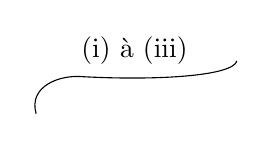
\begin{tikzpicture}[x=1cm,y=1cm]\node at (0,.35) {(i) à (iii)};\draw (-1.25,-.45) .. controls (-1.35,-.1) and (-0.95,.05) .. (-0.65,.02) .. controls (.3,-.03) and (1.25,.03) .. (1.3,.22);\end{tikzpicture}}} sont équivalentes

(i) Les conditions \inserted{\figure{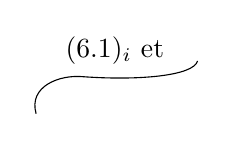
\begin{tikzpicture}[x=1cm,y=1cm]\node at (0,.35) {$(6.1)_i$ et};\draw (-1.0,-.45) .. controls (-1.1,-.1) and (-0.7,.05) .. (-0.4,.02) .. controls (.3,-.03) and (1.0,.03) .. (1.05,.22);\end{tikzpicture}}} $(6.2)_i$ pour tt $i$, et les $\pi_i\in\mathcal E$.

\deleted{\unsure{(ii)} [Une graduation de $\mathcal E^*$ peut être définie par des $\pi'_i$, et pour un \deleted{\illegible{2}} tel choix;]\par
\unsure{(ii)} \unsure{Les conditions} $(6.3)_i$ pour tt $i$ (avec $\pi_i$ \unsure{remplacé par} $\pi'_i$,....)}
\margin{\figure{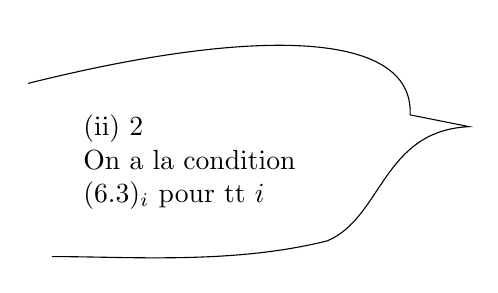
\begin{tikzpicture}[x=1cm,y=1cm]
\node[align=left,text width=4.2cm] at (0,0) {(ii) \deleted{\illegible{2}}\\On a la condition\\$(6.3)_i$ pour tt $i$};
\draw (-2.8,1) .. controls (0,1.7) and (2.1,1.7) .. (2.05,.6) -- (2.8,.45) .. controls (1.7,.4) and (1.7,-.7) .. (1,-1) .. controls (-.2,-1.3) and (-1.5,-1.2) .. (-2.5,-1.2);
\end{tikzpicture}}}

(iii) \deleted{L'hom.}\inserted{On a} \inserted{\figure{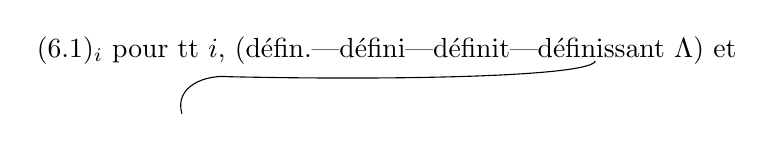
\begin{tikzpicture}[x=1cm,y=1cm]\node at (0,.35) {$(6.1)_i$ pour tt $i$, (\unsure{défin.|défini|définit|définissant} $\Lambda$) et};\draw (-2.6,-.45) .. controls (-2.7,-.1) and (-2.3000000000000003,.05) .. (-2.0,.02) .. controls (.3,-.03) and (2.6,.03) .. (2.65,.22);\end{tikzpicture}}}
\[
\uline{\Lambda\in\mathcal E^{(-2)}}
\tag{6.6}
\]
\deleted{\unsure{(iv)}} Ces conditions impliquent de plus

(iv) Les $\pi_{i,\alpha}$ sont dans $\mathcal E$, \deleted{les $\pi_i$ sont dans $\mathcal E$.}

(v) Les $\pi_i\in\mathcal E$, \inserted{\figure{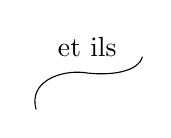
\begin{tikzpicture}[x=1cm,y=1cm]\node at (0,.35) {et ils};\draw (-0.65,-.45) .. controls (-0.75,-.1) and (-0.35000000000000003,.05) .. (-0.050000000000000044,.02) .. controls (.3,-.03) and (0.65,.03) .. (0.7000000000000001,.22);\end{tikzpicture}}} sont \deleted{les seuls projecteurs}\inserted{définis comme formant \inserted{\figure{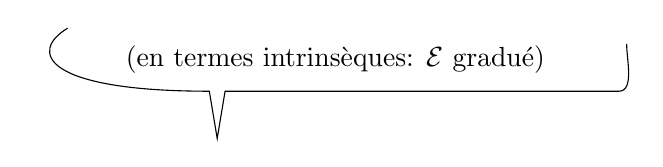
\begin{tikzpicture}[x=1cm,y=1cm]
\node at (0,.3) {(en termes intrinsèques: $\mathcal E$ gradué)};
\draw (-3.4,.7) .. controls (-3.9,.4) and (-3.7,-.1) .. (-1.6,-.1) -- (-1.5,-.7) -- (-1.4,-.1) -- (3.6,-.1) .. controls (3.8,-.1) and (3.7,.3) .. (3.7,.5);
\end{tikzpicture}}}} la seule famille d'éléments de $\mathcal E$ satisfaisant $(1.1.)$ et $(1.3)$ (a) ou b), au choix...., \unsure{$\mathcal E$|\deleted{$\mathcal E$}} ou encore $(1.4)$....).

\deleted{(vi) L'élément $\Lambda$ de $\mathcal E^{(-2)}$ est uniquement déterminé, \deleted{\unsure{par les}} (en termes de \inserted{\figure{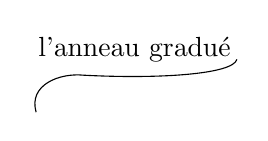
\begin{tikzpicture}[x=1cm,y=1cm]\node at (0,.35) {l'anneau gradué};\draw (-1.25,-.45) .. controls (-1.35,-.1) and (-0.95,.05) .. (-0.65,.02) .. controls (.3,-.03) and (1.25,.03) .. (1.3,.22);\end{tikzpicture}}} $\mathcal E^*$ et l'élt $L\in\mathcal E^{(1)}$, par les conditions suivantes :
\[
\left\{\begin{aligned}
L\Lambda&=1-\sum_{0\leq i\leq n}\pi_{i,0}\\
\Lambda L&=1-\sum_{n\leq i\leq2n}\pi_{i,0}
\end{aligned}\right.
\tag{6.7}
\]}

\uline{Dém.} L'équivalence de (i) et (ii) est claire, et le fait que i est impliqué par (iii) (en prenant $w_i=\Lambda^{\unsure{(}n-i\unsure{)}}$). \deleted{\unsure{Il}}\inserted{\figure{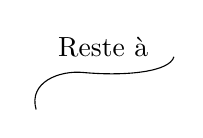
\begin{tikzpicture}[x=1cm,y=1cm]\node at (0,.35) {Reste à};\draw (-0.85,-.45) .. controls (-0.95,-.1) and (-0.55,.05) .. (-0.25,.02) .. controls (.3,-.03) and (0.85,.03) .. (0.9,.22);\end{tikzpicture}}} prouver que (i), (ii) impliquent (iii) à (vi). On \deleted{sait déjà}\inserted{a déjà indiqué} que ça implique \deleted{$(6.7)$} (v).
\mspage{9}
